\section{Semantics}
\label{semantics}

The semantics are divided into two parts: dynamic and static. Dynamic semantic is the same as the evaluation rules in our class, while static semantic includes but not limited to the typing rules. The static semantic also includes some rules to rule out the infinite recursive calling that may be caused by the logical variables introduced by $\lambdaJ$.

As shown in Figure \ref{dynamic-sem-lambdaj}, the $\lambdaJ$ evaluation rules extend {\ensuremath{\lambda}}-calculus evaluation with constraint propagation and symbolic evaluation of logic variables. Evaluation involves keeping track of constraints which are required to be true (hard constraints) and the set of constraints we use for guidance if consistent with our hard constraints (default assumptions). To correctly evaluate conditionals with symbolic conditions, we also need to keep track of the (possibly symbolic) path condition ($\mathscr{G}$). Here, $\Sigma~$stores the current set of constraints, and an environment $\Delta~$stores the set of constraints on default values for logic variables. The rules are no surprising, quite similar to the rules learned in our class. One interesting thing is when evaluating under symbolic conditions, because evaluation of such conditionals with a recursive function application in a branch could lead to infinite recursion when the condition is symbolic. $\lambdaJ$ prevents this anomalous behavior by using the type system.

Static semantic, as shown in Figure \ref{static-sem-lambdaj}, describes simple type-checking and enforce restriction on scope of nondeterminism and recursion. The types are defined in Figure \ref{lambdaj-types}. The largest difference of typing rules between the normal {\ensuremath{\lambda}}-calculus and $\lambdaJ$ is the symbolic values. For int, bool or if expression, it can have two options: concrete or symbolic. And therefore the issue comes when applying reentrant functions under symbolic conditionals. To rule out such kind of cases, $\lambdaJ$ explicitly marks values as concrete or symbolic. For example, a function that might be reentrant should be marked as ($\longrightarrow$). Furthermore, it introduces \textbf{rep}, defined as a predicate that requires that functions taking arguments that may be reentrant be themselves labeled as reentrant. This can help prevent high-order functions from being used to circumvent the restrictions on reentrant calls. Overall, the static semantics can guarantee that
\begin{itemize}
\item concrete values are supplied when concrete values are expected,
\item symbolic values are well-formed,
\item evaluation under symbolic conditions does not cause unexpected infinite recursion,
\item context values have the appropriate types.
\end{itemize}


\begin{figure}
     \begin{spacing}{2.0}
    \fbox{
        \parbox{\textwidth}{
            \begin{center}
                \scriptsize{
                  $ \boxed{\mathscr{G} \vdash \left \langle \Sigma, \Delta, e \right \rangle \rightarrow \left \langle \Sigma', \Delta', e' \right \rangle }$\\}
            \end{center}
            \begin{flushright}
%                \large{
                  $ \frac{
                      \mathscr{G} \vdash \left \langle \Sigma, \Delta, e_1 \right \rangle \rightarrow \left \langle \Sigma', \Delta', e'_1 \right \rangle 
                      }{
                      \mathscr{G} \vdash \left \langle \Sigma, \Delta, e_1~e_2 \right \rangle \rightarrow \left \langle \Sigma', \Delta', e'_1~e_2 \right \rangle 
                      }~~~~\scriptsize{\textrm{E-APP1}}
                      ~~~~~
                      \frac{
                          \mathscr{G} \vdash \left \langle \Sigma, \Delta, e_2 \right \rangle \rightarrow \left \langle \Sigma', \Delta', e'_2 \right \rangle 
                        }{
                        \mathscr{G} \vdash \left \langle \Sigma, \Delta, \upsilon~e_2 \right \rangle \rightarrow \left \langle \Sigma', \Delta', \upsilon~e_2 \right \rangle 
                    }~~~~\scriptsize{\textrm{E-APP2}}$
                    \\
                    $\frac{
                    }{
                    \mathscr{G} \vdash \left \langle \Sigma, \Delta, \lambda x.e~\upsilon \right \rangle \rightarrow \left \langle \Sigma', \Delta', e[x\mapsto \upsilon] \right \rangle 
                    }~~~~\scriptsize{\textrm{E-APPLAMBDA}}
                    ~~~~
                    \frac{
                        c'=c_1~(op)~c_2
                    }{
                    \mathscr{G} \vdash \left \langle \Sigma, \Delta, c_1~(op)~c_2 \right \rangle \rightarrow \left \langle \Sigma', \Delta', c' \right \rangle 
                    }~~~~\scriptsize{\textrm{E-OP}}$
                    \\
                    $\frac{
                        \mathscr{G} \vdash \left \langle \Sigma, \Delta, e_1 \right \rangle \rightarrow \left \langle \Sigma', \Delta', e'_1 \right \rangle 
                    }{
                    \mathscr{G} \vdash \left \langle \Sigma, \Delta, e_1~(op)~e_2 \right \rangle \rightarrow \left \langle \Sigma', \Delta', e'_1~(op)~e_2 \right \rangle 
                    }~~~~\scriptsize{\textrm{E-OP1}}
                    ~~~~
                    \frac{
                        \mathscr{G} \vdash \left \langle \Sigma, \Delta, e_2 \right \rangle \rightarrow \left \langle \Sigma', \Delta', e'_2 \right \rangle 
                    }{
                    \mathscr{G} \vdash \left \langle \Sigma, \Delta, \upsilon~(op)~e_2 \right \rangle \rightarrow \left \langle \Sigma', \Delta', \upsilon~(op)~e'_2 \right \rangle 
                    }~~~~\scriptsize{\textrm{E-OP2}}$
                    \\
                    $\frac{
                        \mathscr{G} \vdash \left \langle \Sigma, \Delta, e_c \right \rangle \rightarrow \left \langle \Sigma', \Delta', e'_c \right \rangle 
                    }{
                    \mathscr{G} \vdash \left \langle \Sigma, \Delta, \textbf{if}~e_c~\textbf{then}~e_t~\textbf{else}~e_f \right \rangle \rightarrow \left \langle \Sigma', \Delta', \textbf{if}~e'_c~\textbf{then}~e_t~\textbf{else}~e_f \right \rangle 
                    }~~~~\scriptsize{\textrm{E-COND}}$
                    \\
                    $\frac{
                        \mathscr{G} \vdash \left \langle \Sigma, \Delta, e_t \right \rangle \rightarrow \left \langle \Sigma', \Delta', e'_t \right \rangle 
                    }{
                        \mathscr{G} \vdash \left \langle \Sigma, \Delta, \textbf{if true}~ \textbf{then}~e_t~\textbf{else}~e_f \right \rangle \rightarrow \left \langle \Sigma', \Delta', e'_t \right \rangle 
                    }~~~~\scriptsize{\textrm{E-CONDTRUE}}$
                    \\
                    $\frac{
                        \mathscr{G} \vdash \left \langle \Sigma, \Delta, e_f \right \rangle \rightarrow \left \langle \Sigma', \Delta', e'_f \right \rangle 
                    }{
                        \mathscr{G} \vdash \left \langle \Sigma, \Delta, \textbf{if false}~\textbf{then}~e_t~\textbf{else}~e_f \right \rangle \rightarrow \left \langle \Sigma', \Delta', e'_f \right \rangle 
                    }~~~~\scriptsize{\textrm{E-CONDFALSE}}$
                    \\
                    $\frac{
                        \sigma\wedge\mathscr{G} \vdash \left \langle \Sigma, \Delta, e_t \right \rangle \rightarrow \left \langle \Sigma', \Delta', e'_t \right \rangle 
                    }{
                        \mathscr{G} \vdash \left \langle \Sigma, \Delta, \textbf{if}~\sigma~\textbf{then}~e_t~\textbf{else}~e_f \right \rangle \rightarrow \left \langle \Sigma', \Delta', \textbf{if}~\sigma~\textbf{then}~e'_t~\textbf{else}~e_f \right \rangle 
                    }~~~~\scriptsize{\textrm{E-CONDSYMT}}$
                    \\
                    $\frac{
                        \neg\sigma\wedge\mathscr{G} \vdash \left \langle \Sigma, \Delta, e_f \right \rangle \rightarrow \left \langle \Sigma', \Delta', e'_f \right \rangle 
                    }{
                        \mathscr{G} \vdash \left \langle \Sigma, \Delta, \textbf{if}~\sigma~\textbf{then}~\upsilon_t~\textbf{else}~e_f \right \rangle \rightarrow \left \langle \Sigma', \Delta', \textbf{if}~\sigma~\textbf{then}~\upsilon_t~\textbf{else}~e'_f \right \rangle 
                    }~~~~\scriptsize{\textrm{E-CONDSYMF}}$          
                    \\
                    $\frac{
                        \mathscr{G} \vdash \left \langle \Sigma, \Delta, e \right \rangle \rightarrow \left \langle \Sigma', \Delta', e' \right \rangle 
                      }{
                          \mathscr{G} \vdash \left \langle \Sigma, \Delta, \textbf{defer}~x:\tau\{e\}~\textbf{default}~\upsilon_d \right \rangle \rightarrow \left \langle \Sigma', \Delta', \textbf{defer}~x:\tau\{e'\}~\textbf{default}~\upsilon_d \right \rangle 
                      }~~~~\scriptsize{\textrm{E-DEFERCONSTRAINT}}$       
                    \\
                    $\frac{
                        fresh~x'
                     }{
                         \mathscr{G} \vdash \left \langle \Sigma, \Delta, \textbf{defer}~x:\tau\{\upsilon_c\}~\textbf{default}~\upsilon_d \right \rangle \rightarrow \left \langle \Sigma\cup\{\mathscr{G}\Rightarrow\upsilon_c[x\mapsto x']\}, \Delta\cup\{\mathscr{G}\Rightarrow x'=\upsilon_d \}, x' \right \rangle 
                     }~~~~\scriptsize{\textrm{E-DEFER}}$       
                    \\
                    $\frac{
                        \mathscr{G} \vdash \left \langle \Sigma, \Delta, e \right \rangle \rightarrow \left \langle \Sigma', \Delta', e' \right \rangle 
                    }{
                        \mathscr{G} \vdash \left \langle \Sigma, \Delta, \textbf{assert}~e \right \rangle \rightarrow \left \langle \Sigma', \Delta', \textbf{assert}~e' \right \rangle 
                    }~~~~\scriptsize{\textrm{E-ASSERTCONSTRAINT}} $
                    \\
                    $\frac{ 
                    }{
                        \mathscr{G} \vdash \left \langle \Sigma, \Delta, \textbf{assert}~\upsilon \right \rangle \rightarrow \left \langle \Sigma\cup\{\mathscr{G}\Rightarrow\upsilon\}, \Delta, () \right \rangle 
                    }~~~~\scriptsize{\textrm{E-ASSERT}}$   
                    \\
                    $\frac{
                        \mathscr{G} \vdash \left \langle \Sigma, \Delta, e \right \rangle \rightarrow \left \langle \Sigma', \Delta', e' \right \rangle 
                    }{
                        \mathscr{G} \vdash \left \langle \Sigma, \Delta, \textbf{concretize}~e~\textbf{with}~\upsilon_c \right \rangle \rightarrow \left \langle \Sigma', \Delta', \textbf{concretize}~e'~\textbf{with}~\upsilon_c \right \rangle 
                    }~~~~\scriptsize{\textrm{E-CONCRETIZEEXP}}$   
                    \\
                    $\frac{
                        \textrm{MODLE}( \Delta, \Sigma\cup\{\mathscr{G}\cap\textbf{context}=\upsilon_c \})=\mathscr{M}~~~c=\mathscr{M}[[\upsilon_\nu]]
                    }{
                        \mathscr{G} \vdash \left \langle \Sigma, \Delta, \textbf{concretize}~\upsilon_\nu~\textbf{with}~\upsilon_c \right \rangle \rightarrow \left \langle \Sigma, \Delta, c \right \rangle 
                    }~~~~\scriptsize{\textrm{E-CONCRETIZESAT}}$   
                    \\
                    $\frac{
                        \textrm{MODLE}( \Delta, \Sigma\cup\{\mathscr{G}\cap\textbf{context}=\upsilon_c \})=\textrm{UNSAT}
                    }{
                        \mathscr{G} \vdash \left \langle \Sigma, \Delta, \textbf{concretize}~\upsilon_\nu~\textbf{with}~\upsilon_c \right \rangle \rightarrow \left \langle \Sigma, \Delta, \textbf{error} \right \rangle 
                    }~~~~\scriptsize{\textrm{E-CONCRETIZEUNSAT}}$   
%                }
           \end{flushright}
        }
    }
\end{spacing}
    \caption{Dynamic semantics for $\lambdaJ$.}
    \label{dynamic-sem-lambdaj}
\end{figure}

   \begin{figure}[!htbp]
       \fbox{%  
           \parbox{\textwidth}{%  
               \begin{center}  
                   \begin{align*}
                   \delta~:: = ~ & {\begin{aligned}[t]
                       & ~ \textbf{concretize}~|~\textbf{sym}
                       ~~~~~~~~
                       ~~~~~~~~~~~~~~~\textrm{determinism tag}                  
                       \end{aligned}}\\
                    \beta~:: = ~ & {\begin{aligned}[t]
                        & ~ \textbf{int}_c~|~\textbf{bool}_c~|~\textbf{unit}~| ~ \textbf{int}~|~\textbf{bool}
                        ~~~~~~~~~~~~~~~\textrm{base type}
                        \end{aligned}}\\
                    \tau~:: = ~ & {\begin{aligned}[t]
                        & ~ \beta~|~\tau_1 \stackrel{nr}{\longrightarrow} \tau_2~|~\tau_1\rightarrow\tau_2
                        ~~~~~~~~~~~~~~~~~~~
                        ~~~~~~~~~~~~~~~\textrm{type}
                        \end{aligned}}
                    \end{align*}
                \end{center}  
            }%  
        }
        \caption{$\lambdaJ$ types}
        \label{lambdaj-types}
    \end{figure}

\begin{figure}
    \begin{spacing}{2.0}
        \fbox{
            \parbox{\textwidth}{
                \begin{center}
                    \scriptsize{
                        $ \boxed{\tau_1<:\tau_2}$}
                \end{center}
                \begin{flushright}
                    $ \frac{
                    }{
                        \tau<:\tau
                    }~~~~\scriptsize{\textrm{S-REFLEXIVE}}
                    ~~~~~
                    \frac{
                    }{
                        \textbf{int}_c<:\textbf{int}
                    }~~~~\scriptsize{\textrm{S-INT}}
                    ~~~~~
                    \frac{
                    }{
                    \textbf{bool}_c<:\textbf{bool}
                    }~~~~\scriptsize{\textrm{S-BOOL}}$
                    \\
                    $\frac{
                    }{
                    \tau_1 \stackrel{nr}{\longrightarrow} \tau_2<:\tau_1\rightarrow\tau_2
                    }~~~~\scriptsize{\textrm{S-RECFUN}}
                    ~~~~~
                    \frac{
                        \tau'_1<:\tau_1~~\tau_2<:\tau'_2
                    }{
                    \tau_1 \rightarrow \tau_2 <: \tau'_1 \rightarrow \tau'_2
                    }~~~~\scriptsize{\textrm{S-FUN}} $
                    \\
                \end{flushright}
                \begin{center}
                    \scriptsize{
                        $ \boxed{\textbf{rep}~\tau}$}
                \end{center}
                \begin{flushright}
                    $ \frac{
                        \textbf{rep}~\tau~~~\tau'<:\tau
                    }{
                        \textbf{rep}~\tau
                    }~~~~\scriptsize{\textrm{OK-SUBTYPE}}
                    ~~~~~
                    \frac{
                    }{
                        \textbf{rep}~\beta
                    }~~~~\scriptsize{\textrm{OK-BASETYPE}}$
                    \\
                    $\frac{
                        \textbf{rep}~\tau_2
                    }{
                    \textbf{rep}~\beta_1 \rightarrow \tau_2
                    }~~~~\scriptsize{\textrm{OK-BASEFUNCTION}}
                    ~~~~~
                    \frac{
                        \textbf{rep}~(\tau_1 \stackrel{nr}{\rightarrow}\tau')~~\textbf{rep}~\tau_2
                    }{
                        \textbf{rep}~(\tau_1 \stackrel{nr}{\rightarrow}\tau') \stackrel{nr}{\rightarrow} \tau_2
                    }~~~~\scriptsize{\textrm{OK-HOFUNCTION}}$
                    \\
                    $\frac{
                        \textbf{rep}~\tau_1\rightarrow \tau_2
                    }{
                        \textbf{rep}~(\tau_1\rightarrow \tau_2) \rightarrow\beta
                    }~~~~\scriptsize{\textrm{OK-RECFUNCTIONBASE}}
                    ~~~~~
                    \frac{
                        \textbf{rep}~\tau_1 \rightarrow \tau_2~~\textbf{rep}~\tau'_1 \rightarrow \tau'_2
                    }{
                        \textbf{rep}~(\tau_1 \rightarrow \tau_2) \rightarrow (\tau'_1 \rightarrow \tau'_2)
                    }~~~~\scriptsize{\textrm{OK-RECFUNCTION}}$
                    \\
                \end{flushright}
                \begin{center}
                    \scriptsize{
                        $ \boxed{\Gamma;\gamma\vdash e:\left\langle \tau, \delta \right\rangle }$}
                \end{center}
                \begin{flushright}
                    $ \frac{
                        x\in \Gamma
                    }{
                        \Gamma;\gamma\vdash x:\Gamma(x)
                    }~~~~\scriptsize{\textrm{T-VAR}}
                    ~~~~~
                    \frac{
                    }{
                        \Gamma;\gamma\vdash n:\textbf{int}_c
                    }~~~~\scriptsize{\textrm{T-INT}}
                    ~~~~~
                    \frac{
                    }{
                    \Gamma;\gamma\vdash b:\textbf{bool}_c
                    }~~~~\scriptsize{\textrm{T-BOOL}}
                    ~~~~~
                    \frac{
                    }{
                    \Gamma;\gamma\vdash ():\textbf{unit}
                    }~~~~\scriptsize{\textrm{T-UNIT}}$
                    \\
                    $\frac{
                        \textbf{rep}~\tau
                    }{
                    \Gamma;\gamma\vdash \textbf{context}~\tau :\tau
                    }~~~~\scriptsize{\textrm{T-CONTEXT}}
                    ~~~~~
                    \frac{
                        \Gamma;\gamma\vdash e_1 :\tau_1~~
                        \Gamma;\gamma\vdash e_2 :\tau_2~~
                        \tau_1,\tau_2 <:\tau~~
                        \textbf{rep}~\tau
                    }{
                        \Gamma;\gamma\vdash e_1~(op)~e_2 :\tau
                    }~~~~\scriptsize{\textrm{T-OP}}$
                    \\
                    $ \frac{
                        \Gamma;\gamma\vdash e :\textbf{bool}_c~~
                        \Gamma;\gamma\vdash e_t :\tau_1~~
                        \Gamma;\gamma\vdash e_f :\tau_2~~
                        \tau_1,\tau_2 <:\tau~~
                        \textbf{rep}~\tau
                    }{
                    \Gamma;\gamma\vdash \textbf{if}~e~\textbf{then}~e_t~\textbf{else}~e_f :\tau
                }~~~~\scriptsize{\textrm{T-CONDC}}$
                \\
                $ \frac{
                     \Gamma;\gamma\vdash e :\textbf{bool}~~
                     \Gamma;\textbf{sym} \vdash e_t :\beta_1~~
                     \Gamma;\textbf{sym} \vdash e_f :\beta_2~~
                      \beta_1,\beta_2 <:\beta_c~~
                     \textbf{rep}~\beta_c
                    }{
                    \Gamma;\gamma\vdash \textbf{if}~e~\textbf{then}~e_t~\textbf{else}~e_f :\beta_c
                }~~~~\scriptsize{\textrm{T-CONDSYM}}$
                \\
                $ \frac{
                    \Gamma,x:\tau_d;\gamma\vdash e :\tau'~~
                    \textbf{rep}~\tau_d~~
                    \textbf{rep}~\tau'
                }{
                    \Gamma;\gamma\vdash (\lambda x:\tau_d.e):\tau_d\rightarrow \tau'
                }~~~~\scriptsize{\textrm{T-LAMBDA}}
                ~~~~~
                 \frac{
                     \Gamma;\gamma\vdash e_1:\tau_1\stackrel{nr}{\rightarrow}\tau_2~~
                     \Gamma,x:\tau_d;\gamma\vdash e_2 :\tau'_1~~
                     \tau'_1<:\tau_1~~
                     \textbf{rep}~\tau_1~~
                     \textbf{rep}~\tau_2
                    }{
                    \Gamma;\gamma\vdash (e_1~e_2):\tau_2
                }~~~~\scriptsize{\textrm{T-APP}}$
                \\
                $\frac{
                    \Gamma,f:\tau_1 \rightarrow \tau_2 ;\gamma\vdash e_1:\tau_1 \rightarrow \tau_2~~
                    \Gamma,f:\tau_1 \stackrel{nr}{\rightarrow} \tau_2 ;\gamma\vdash e_2:\tau_2~~
                    \textbf{rep}~\tau~~
                    \textbf{rep}~\tau_2
                }{
                    \Gamma;\gamma\vdash \textbf{let rec}~f:\tau_1 \stackrel{nr}{\rightarrow} \tau_2=e_1~\textbf{in}~e_2:\tau_2
                }~~~~\scriptsize{\textrm{T-APPLETREC}}$
                \\
                $\frac{
                    \gamma=\textbf{concrete}~~
                    \Gamma;\gamma\vdash e_1:\tau_1 \rightarrow \tau_2~~
                    \Gamma;\gamma\vdash e_2:\tau'_1~~
                    \tau'_1<:\tau_1~~
                    \textbf{rep}~\tau_1~~
                    \textbf{rep}~\tau_2
                }{
                    \Gamma;\gamma\vdash (e_1~e_2):\tau_2
                }~~~~\scriptsize{\textrm{T-APPCURREC}}$
                 \\
                 $ \frac{
                     \Gamma,x:\beta;\gamma\vdash e_c :\textbf{bool}~~
                     \Gamma;\gamma\vdash \upsilon :\beta
                    }{
                        \Gamma;\gamma\vdash (\textbf{defer} x:\beta\{e_c\}~\textbf{default}~\upsilon):\beta
                    }~~~~\scriptsize{\textrm{T-DEFER}}
                    ~~~~~
                    \frac{
                        \Gamma;\gamma\vdash e_c:\textbf{bool}~~
                    }{
                        \Gamma;\gamma\vdash (\textbf{assert}~e_c):\textbf{unit}
                    }~~~~\scriptsize{\textrm{T-ASSERT}}$
                    \\
                    $\frac{
                        \Gamma;\gamma\vdash e_1:\beta~~
                        \Gamma;\gamma\vdash^{c} e_1:\beta'~~
                        \Gamma;\gamma\vdash \upsilon:\beta'
                    }{
                    \Gamma;\gamma\vdash (\textbf{concretize}~e_1~\textbf{with}~\upsilon):\beta_c
                }~~~~\scriptsize{\textrm{T-CONCRETIZE}}$
                \end{flushright}
               }
           }
\end{spacing}
\caption{Static semantics for $\lambdaJ$ describing simple type-checking and enforce restriction on scope of nondeterminism and recursion. Recall that $\beta$ refers to base (non-function) types.}
\label{static-sem-lambdaj}
\end{figure}

\begin{figure}
    \centering
    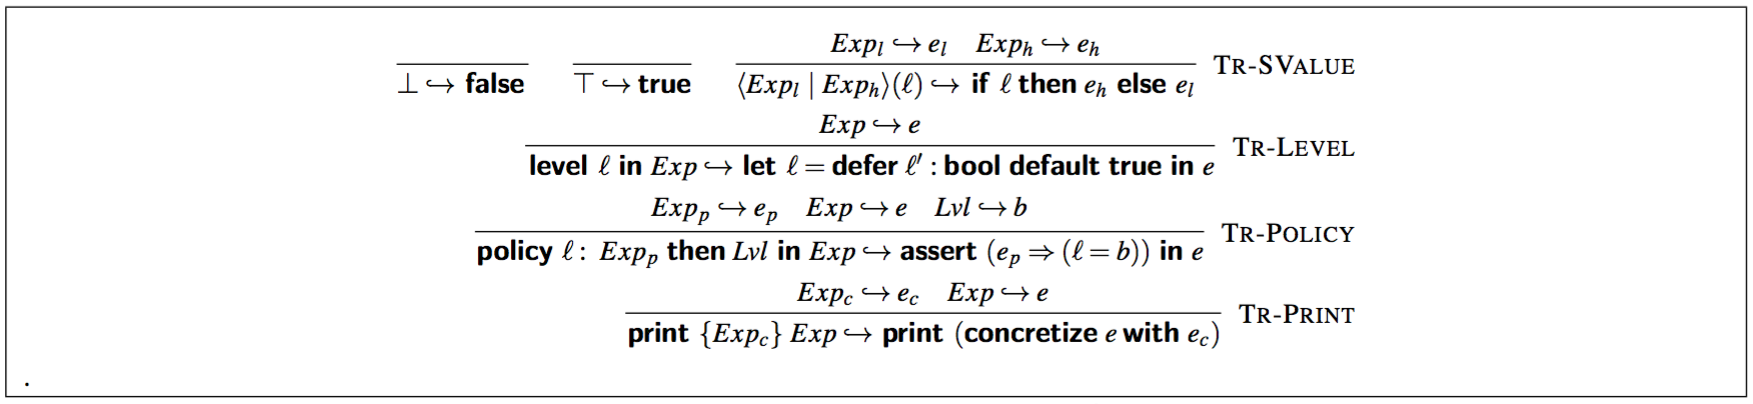
\includegraphics[width=1.0\textwidth]{trans.PNG}
    %\vspace*{-.6cm}
    \caption{Translation from Jeeves to $\lambdaJ$}
    \label{fig:AndroidFUSE}
\end{figure}